
\documentclass[12pt]{book}
\usepackage{cclicenses}
\usepackage[letterpaper,  hmargin = { 1in},vmargin = { 1in}]{geometry}
\usepackage{hyperref}
\usepackage[T1]{fontenc}
\usepackage{multicol}
\newcommand{\mytitle}{Scivault Physics}
\usepackage{amsmath}
\usepackage{cleveref}
\usepackage{longtable}
\usepackage{appendix}
\usepackage{makeidx}
\usepackage{tikz}
\usepackage[linewidth=1pt]{mdframed}
\setlength{\columnsep}{1cm}

\makeindex

%%% To make index work,
% 1) Compile
%2) From base directory, run:
%   makeindex "Scivault Physics.idx"
%3) Compile again

\begin{document}
	\frontmatter
	\title{\mytitle}
	\author{Jonas Williamson}
	\date{Version \the\year\the\month\the\day}
	\maketitle

\normalsize
	\copyright \space \the\year\space by Jonas Williamson.  All Rights Reserved. 
	
		\vspace{2 in}	


	\vspace{1 in}

	\tableofcontents


\mainmatter


	
	
	
	
	
	

	
	


\chapter{Introduction}
\section{Dimensional Analysis and SI units}
\subsection{SI Units}
The \textbf{SI}\index{SI system of units} system of units is the standard used by many scientists throughout the world.  There are seven \textit{fundamental} or \textit{base} quantities from which all other measurements are derived.  These quantities are listed below:
 \index{Units, Fundamental}

\begin{center}

	
\begin{table}[ht]\caption{\textbf{SI Units}}% title of Table 
	\centering % used for centering table	
	\begin{tabular}{|c|c|c|}
		\hline \hline
		\textbf{Quantity} & \textbf{Unit} & \textbf{Unit Symbol}\\
		\hline
		time & second & s \\
		\hline
		length & meter & m \\
		\hline
		mass & kilogram & kg \\
		\hline
		electrical current & Ampere & A \\
		\hline
		temperature & Kelvin & K \\
		\hline
		amount of substance & mole & mol \\
		\hline
		luminous intensity & candela & cd \\
		\hline		
	\end{tabular}
	\label{table:nonlin}% is used to refer this table in the text
\end{table}
\end{center}

	Of these quantities, mass, time and length are quite common.  Thus, this system is sometimes called the MKS (meter, kilogram, second) system. In order to use any equations, all measurements must have correct units.  For example, if a time is expressed in hours, it must first be converted into seconds before any calculations can be attempted.  
	
	\subsection{Dimensional Analysis}
	Dimensional analysis \index{Dimensional Analysis} is the process in which the units associated with quantities create \textit{derived units}. \index{Units, Derived} For instance, when a distance is divided by a time, the units will be $ \frac{m}{s}$ (read \textit{meters per second}).  	
	
	Dimensional analysis is an important part of solving physics problems.  Often, correct dimensional analysis can help you determine if a problem has been solved correctly.  One should not even attempt to calculate an answer to a problem until the correct units have been verified. 

	\subsection{Unit Conversions} \index{Unit Conversions}
	Often you will find that you need to convert a measurement from one unit to another.  In order to do this, you must use a \textit{conversion factor.}  A conversion factor is a fraction that is based upon a statement of equality.  For instance, since 60 seconds = 1 minute, a conversion factor will look like either $\frac{60s}{1 min}$ or $\frac{1 min}{60s}$.  You should chose the version of the conversion factor that eliminates the units that you wish to convert.  
	
	
		\begin{mdframed}[backgroundcolor=blue!10!white]
		\begin{center}
			\textbf{Example \thesubsection}	\label{ex113}
		\end{center}
	
		\vspace{0.1in}	
		\textbf{Problem:} Convert 7.241 hours into seconds. 
		\vspace{0.1in}
		
		\textbf{Solution:} Begin by converting 7.241 hours into minutes.  Since 60 minutes = 1 hour, 
			\begin{equation*}
			7.241 \cancel{hr} \frac{60 min}{1 \cancel{hr}} = 434.46 min
			\end{equation*}
		
		Knowing that 1 minute = 60 seconds, we can use a second conversion factor to obtain seconds:
			\begin{equation*}
			434.46 \cancel{min} \frac{60 s}{1 \cancel{min}} = \boxed{26067.6s}
			\end{equation*}
		
		This problem could be solved in one step if you know that 1 hour = 3600 seconds. 
	
	\end{mdframed}


	
\begin{mdframed}[backgroundcolor=blue!10!white]
	\begin{center}
		\textbf{Example \thesubsection.2}	\label{ex1132}
	\end{center}
	
	\vspace{0.1in}	
	\textbf{Problem:} A car travels with a speed of 20 m/s.  What is this in miles per hour? 
	\vspace{0.1in}
	
	\textbf{Solution:} We begin by converting meters per second into meters per hour:
	\begin{equation*}
	20 \frac{m}{\cancel{s}} \cdot \frac{3600 \cancel{s}}{1 {hr}} = 72000 \frac{m}{hr}
	\end{equation*}
	
	We also need to know that 1 mile = 1609.34 meters:
	\begin{equation*}
		72000 \frac{\cancel{m}}{hr} \cdot \frac{1 mile}{1609.34 \cancel{m}} \approx 44.739 \frac{miles}{hr} 
	\end{equation*}
	
	
\end{mdframed}
		


\section{Vectors and Scalars}
In the study of physics, there are two types of quantities that we will deal with on a regular basis: \textit{scalars} and \textit{vectors}.  

A \textbf{scalar} is a quantity that you are already most likely very familiar with, as it is just a number; scalars have only a \textit{magnitude} (a number that represents how big or strong it is), and can sometimes include units.  Examples of scalars might be the number of people in a room, the mass of a car, or your age in years.  

\textbf{Vectors} are different from scalars because in addition to a magnitude, they contain a direction as well.  Examples of vectors might include 50 feet to the north, 5 m/s at a 33$^\circ$ angle, or 200 miles straight up.  
There are many ways of expressing vectors.  Symbollically, they are often written with an arrow over them.  For example, in the equation \color{blue} $\vec{F} = m \vec{a}$ \color{black}  both force and acceleration are vectors - meaning that both force and acceleration have a direction.  Sometimes vectors will be expressed in \textbf{bold} typeface.   Hence, the expression \\ \color{blue} \textbf{F} = m \textbf{a}  \color{black} is equivalent to the expression shown above.

The direction for vectors in 1 dimension is easy - all you need is a positive or a negative.  Usually, 1-dimensional motion takes place along the x-axis (left and right), but sometimes it will take place in the y- (forward and backward) and z- (up and down) dimensions.  For the purposes of this book, positive is to the right and up unless otherwise stated. 
In two dimensions, a vector requires two pieces of information.  One way of expressing a vector is in polar form.  Polar form in two dimensions includes a magnitude of the vector and an angle, usually measured from the x-axis.  There are several ways for writing this.  4 cm @ 15$^\circ$, \\ 4 cm $\angle 15^\circ$ and 4 cm at 15$^\circ$ North of East all represent the following displacement vector:



\begin{figure}[h]
	\caption{A vector represented graphically.} \label{figure:M1}
	\centering
	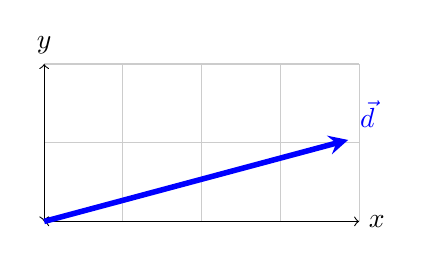
\begin{tikzpicture}
	
	\draw[thin,gray!40] (0,0) grid (4,2);
	\draw[<->] (0,0)--(4,0) node[right]{$x$};
	\draw[<->] (0,0)--(0,2) node[above]{$y$};
	\draw[line width=2pt,blue,-stealth](0,0)--(3.86,1.035) node[anchor=south west]{$\vec{d}$};
	
	
	
	
	\end{tikzpicture}
	
\end{figure}


	
	
	



	
	The magnitude of the above vector is 4 cm.  Mathematically, the magnitude of a vector can be written several ways, the most common being $\lvert \vec{A} \rvert$, though sometimes the magnitude of a vector can be written as the vector without the vector sign, as in $A$. 
	
	Unit vectors are vectors that have a length of one unit and are oriented along one axis.  The unit vector for the x-direction is written as $\hat{i}$ (pronounced i-hat).  $\hat{i}$ is a 1-unit long vector that is always parallel to the x-axis, and points in the direction of increasing x values.  Likewise, the y-direction and z-direction unit vectors are written as $\hat{j}$ and $\hat{k}$ respectively.  
	
	
	Because the surface of a paper is effectively 2-dimensional, it is very hard to draw lines that are oriented directly into or out of your paper. For this purpose, physicists have agreed to the following convention: vectors that point directly into your paper are notated by $\bigotimes$ .  Vectors that point directly out of your paper are shown by the symbol $\bigodot$.  
	
	Sometimes, vectors may be expressed in Cartesian coordinates.  This vector could either be expressed as an ordered pair (or triple) with square brackets, such as [3, 4, 5] cm, or as a linear combination of the unit vectors shown above, such as $5\hat{i} + 12 \hat{j} + 3 \hat{k}$  In each case, the distances in each direction are given by the numbers shown.  The vector in figure \ref{figure:M1} could be represented as: \color{blue} $\vec{d}  \approx 3.86 \hat{i} + 1.035 \hat{j}$.  \color{black}
	
	When converting between polar and cartesian forms for two dimensional vectors, a little trigonometry shows: 
		\begin{mdframed}[backgroundcolor=orange!20!white]
	
	\color{blue}
	\begin{multicols}{2}
		\begin{center}
			\begin{equation}
			x = r \cos(\theta)
			\label{eq11}
			\end{equation}
			
			\begin{equation}
			y = r \sin(\theta)
			\end{equation}

			\begin{equation}
			r = \sqrt{x^2+y^2}			
			\end{equation}

			\begin{equation}
			\theta=\tan^{-1}(\frac{y}{x})
			\label{eq14}
			\end{equation}		
		\end{center}
	\end{multicols}
	\color{black}
	\end{mdframed}
	
	In three dimensions, polar form comes in two types: \textbf{cylindrical} and \textbf{spherical}.  In cylindrical coordinates, expressed as [r, $\theta$, z],  the above conversions are used, and the z-coordinate remains unchanged from Cartesian form.  In spherical coordinates, the vector [r, $\theta$, $\phi$] includes a radial distance, an azimuthal angle and a polar angle. 

	
	
	
	
\section{Vector Mathematics}
	\subsection{Vector Addition} \index{Vectors, Addition}
	\subsubsection{Graphical Addition of Vectors} 
	When vectors are added graphically, they are added \textbf{head} to \textbf{tail}.  This means that the arrowhead for a first vector becomes the origin for the second vector.  The \textbf{resultant} vector is a straight line between the origin of the first vector and the head of the second.  
	
	
	\begin{mdframed}[backgroundcolor=blue!10!white]
		\begin{center}
			
			
			\textbf{Example \thesubsection}	\label{test}
		\end{center}
		
		\vspace{0.1in}
		\textbf{Problem:}  If $\vec{A} =  \hat{i} + 2 \hat{j} $ and $\vec{B} = 3 \hat{i} - \hat{j} $, 
		find $\vec{C}$ graphically given $\vec{C} = \vec{A} + \vec{B}$ 
		
		\vspace{0.1in}
		
		
		\textbf{Solution:} Begin by drawing $\vec{A}$:
		
		
			
		
		\begin{center}
			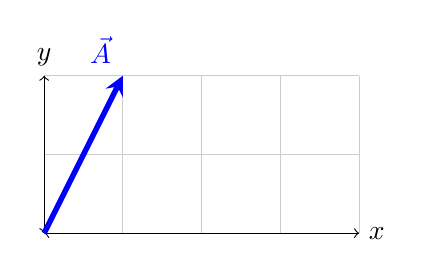
\begin{tikzpicture}
			\draw[thin,gray!40] (0,0) grid (4,2);
			\draw[<->] (0,0)--(4,0) node[right]{$x$};
			\draw[<->] (0,0)--(0,2) node[above]{$y$};
			\draw[line width=2pt,blue,-stealth](0,0)--(1,2) node[anchor=south east]{$\vec{A}$};

			\end{tikzpicture}
			
		\end{center}
	
		Now use the head of $\vec{A} $ as the origin for $\vec{B}$:
	
	
		\begin{center}
		
		
		
		
		
		
		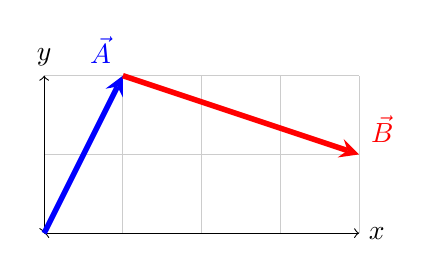
\begin{tikzpicture}
		\draw[thin,gray!40] (0,0) grid (4,2);
		\draw[<->] (0,0)--(4,0) node[right]{$x$};
		\draw[<->] (0,0)--(0,2) node[above]{$y$};
		\draw[line width=2pt,blue,-stealth](0,0)--(1,2) node[anchor=south east]{$\vec{A}$};
		\draw[line width=2pt,red,-stealth](1,2)--(4,1) node[anchor=south west]{$\vec{B}$};

		\end{tikzpicture}		
		
	\end{center}
	
	The resulting vector is a straight line from the origin to the end of $\vec{B}$: 
	
	
	\begin{center}
		

		
		
		
		
			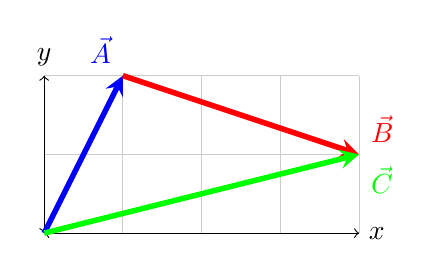
\begin{tikzpicture}
			\draw[thin,gray!40] (0,0) grid (4,2);
			\draw[<->] (0,0)--(4,0) node[right]{$x$};
			\draw[<->] (0,0)--(0,2) node[above]{$y$};
			\draw[line width=2pt,blue,-stealth](0,0)--(1,2) node[anchor=south east]{$\vec{A}$};
			\draw[line width=2pt,red,-stealth](1,2)--(4,1) node[anchor=south west]{$\vec{B}$};
			\draw[line width=2pt,green,-stealth](0,0)--(4,1) node[anchor=north west]{$\vec{C}$};
			\end{tikzpicture}
			
			
			
		\end{center}
		
		The resultant vector is given by $\boxed {\vec{C} = 4 \hat{i} + \hat{j}}$
		
	\end{mdframed}
	
	\subsubsection{Mathematical Addition of Vectors}
	Mathematical addition of vectors in Cartesian form is quite easy - simply add corresponding x- and y- values together.  For instance, in Example \ref{test} we are given  $\vec{A} =  \hat{i} + 2 \hat{j} $ and $\vec{B} = 3 \hat{i} - \hat{j} $.  Adding these together would give $\vec{C} = (1 +3) \hat{i} + (2-1)\hat{j} \longrightarrow \vec{C} =  4 \hat{i} + \hat{j} $.
	
	The easiest way to add vectors that are expressed in polar coordinates is to first convert them into cartesian coordinates using Equations \eqref{eq11} through \eqref{eq14} on page \pageref{eq11}.
	
	
	
	\subsection{The Dot Product} \index{Dot Product} \index{Vectors, Dot Product}
	\subsubsection{In Cartesian Form}
	When multiplying vectors, it is sometimes necessary to obtain a scalar result.  This is done through use of a dot product.  A dot product is written as $\vec{A} \cdot \vec{B} $.  This means to only multiply the components of the vectors that are in the same direction.  In cartesian coordinates, this can be done by multiplying corresponding components, then adding the products.  
	
		\begin{mdframed}[backgroundcolor=blue!10!white]
			\begin{center}
				\textbf{Example \thesubsection}	\label{example:dotproduct}
				
				
			\end{center}
		
		\textbf{Problem:} Given the vectors $ \vec{Y} = 2 \hat{i} + 3 \hat{j} $ and $\vec{Z} = -4 \hat{i} + 5 \hat{j}$ find the dot product of vectors Y and Z. 
		
		\vspace{.1in}
		
		\textbf{Solution:} Multiply coefficients from each vector, then add the products together:
		\begin{center}
			$2\times(-4) + 3\times 5 = -8 + 15 = \boxed{7}$ 
		\end{center}
		
		
		\end{mdframed}
	\subsubsection{In Polar Form}
	Often, vectors will be expressed in polar notation.  If this is the case, the dot product can be found my multiplying the magnitude of the first vector times the magnitude of the second vector times the cosine of the angle between:
	
	
	\begin{mdframed}[backgroundcolor=orange!20!white]
		\begin{equation}
			\label{equation:dotproduct}
		\vec{A} \cdot \vec{B} = \lvert \vec{A} \rvert  \lvert \vec{B} \rvert \cos{\theta}
		\end{equation}
		
	\end{mdframed}
	
	
	\vspace{0.1in}
	
	
		\begin{mdframed}[backgroundcolor=blue!10!white]
		\begin{center}
			\textbf{Example \thesubsection.2}	\label{example:dotproduct2}
			\vspace{0.1in}
			
			
		\end{center}
		
		\textbf{Problem:} Given the vectors $ \vec{D} = 3 \angle 30^{\circ} $ and $\vec{E} = 5 \angle 60^{\circ}$ find the dot product of vectors D and E. 
		
		\vspace{.1in}
		
		\textbf{Solution:}  We begin by graphing both vectors starting from a common origin:
		\begin{center}
		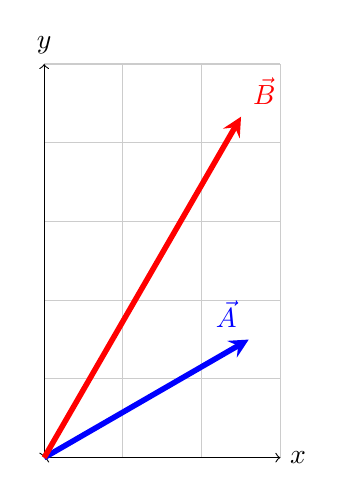
\begin{tikzpicture}
		\draw[thin,gray!40] (0,0) grid (3,5);
		\draw[<->] (0,0)--(3,0) node[right]{$x$};
		\draw[<->] (0,0)--(0,5) node[above]{$y$};
		\draw[line width=2pt,blue,-stealth](0,0)--(2.598,1.5) node[anchor=south east]{$\vec{A}$};
		\draw[line width=2pt,red,-stealth](0,0)--(2.5,4.33) node[anchor=south west]{$\vec{B}$};
		
		\end{tikzpicture}	
			

		\end{center}
			
			Noticing that the angle between the two vectors is $30^\circ$, we can use equation 1.5 to calculate:
			
			\begin{center}
				$ 		\vec{D} \cdot \vec{E} = \lvert \vec{D} \rvert  \lvert \vec{E} \rvert \cos{\theta} = (3)(5)\cos30^\circ \approx \boxed{12.990} $
			\end{center}
		
		
		
		
		\begin{center}
			
		\end{center}
		
		
	\end{mdframed}
	
	
	
	\subsection{The Cross Product}  \index{Cross Product} \index{Vectors, Cross Product}
	\subsubsection{Cross Products In Cartesian Form}
	Sometimes two vectors will be multiplied in such a way that they will result in another vector.  This is called a \textbf{Cross Product}.  A cross product is inherently a three-dimensional operation.  A cross product can be found by calculating the determinant of a matrix:  
	
\begin{mdframed}[backgroundcolor=orange!20!white]
\begin{equation}
 \vec{A} \times \vec{B} = 	\begin{vmatrix}
				\hat{i} & \hat{j} & \hat{k}\\
				A_x & A_y & A_z \\
				B_x & B_y & B_z 
				\end{vmatrix} 
				\label{equation:16}
\end{equation}
\end{mdframed}	

	
The most common way to find the determinant of the above matrix is by using minors:
\begin{center}
$
 \vec{A} \times \vec{B} = 	\begin{vmatrix}
	\hat{i} & \hat{j} & \hat{k}\\
	A_x & A_y & A_z \\
	B_x & B_y & B_z 
\end{vmatrix} 
= \hat{i} \begin{vmatrix}
	A_y & A_z \\
	B_y & B_z 
\end{vmatrix} - \hat{j} \begin{vmatrix}
A_x & A_z \\
B_x & B_z 
\end{vmatrix} + \hat{k} \begin{vmatrix}
A_x & A_y \\
B_x & B_y 
\end{vmatrix}
$
\end{center}

This finding the determinate of each of the 2x2 matrices yields:
\begin{center}
	$ \vec{A} \times \vec{B} = 	\hat{i} (A_y B_z - A_z B_y) - \hat{j}(A_x B_z - A_z B_x)+ \hat{k}(A_x B_y - A_y B_x)
$\end{center}



	\begin{mdframed}[backgroundcolor=blue!10!white]
	\begin{center}
		\textbf{Example \thesubsection}	\label{example:crossproductcartesian}
		\vspace{0.1in}
		
		
	\end{center}
	
	\textbf{Problem:} Given the vectors $ \vec{V} = 2 \hat{i} + 3 \hat{j} $ and $\vec{W} = -4 \hat{i} + 5 \hat{j}$ find the cross product of vectors V and W. 
	
	\vspace{.1in}
	
	\textbf{Solution:}  Begin by creating a matrix, as shown in equation \eqref{equation:16}.  Since both vectors lie in the X-Y plane, the Z-components for both vectors are zero:
	
	\begin{center}
		$\vec{V} \times \vec{W} =  \begin{vmatrix}
		\hat{i} & \hat{j} & \hat{k} \\
		2 & 3 & 0\\
		-4 & 5 & 0		
		\end{vmatrix}$

	\end{center}

Now, use expansion by minors to create three two-by-two matrices:

\begin{center}
	$\vec{V} \times \vec{W} =  \begin{vmatrix}
	\hat{i} & \hat{j} & \hat{k} \\
	2 & 3 & 0\\
	-4 & 5 & 0		
	\end{vmatrix} = \hat{i} \begin{vmatrix}
		3 & 0 \\
		5 & 0 
	\end{vmatrix} - \hat{j} \begin{vmatrix}
		2 & 0 \\
		-4 & 0 
	\end{vmatrix} + \hat{k} \begin{vmatrix}
		2 & 3 \\
		-4 & 5 
	\end{vmatrix}
	$
\end{center}

Finding the determinate of each of the two-by-two matricies yields: 
\begin{center}
	$	\vec{V} \times \vec{W} = \hat{i}(3\cdot0-0\cdot5)-\hat{j}(2\cdot0-0\cdot(-4))+\hat{k}(2\cdot5-3\cdot(-4))$
\end{center}

Both the x-component and the y-components of this cross product are zero.  Thus, 
\begin{center}
	$	\boxed{\vec{V} \times \vec{W} = 22 \hat{k}}$
\end{center}


\end{mdframed}
	
	There are some important things you may wish to note.  
	\begin{enumerate}
		\item The cross product is not commutative.  That is, $\vec{A} \times \vec{B} \neq \vec{B} \times \vec{A}$.  In fact, the two cross products are in exactly opposite directions.  
		\item The cross product of two vectors is always a vector that is perpendicular to both of the original vectors.  
	\end{enumerate}


\subsubsection{Cross Products In Polar Form}
	When vectors are expressed in polar form, a cross product can often be found using two steps.  To find the magnitude of the resulting vector, one would use the following equation:
	
\begin{mdframed}[backgroundcolor=orange!20!white]
	\begin{equation}
	\lvert \vec{A} \times \vec{B} \rvert = 	\lvert \vec{A} \rvert \lvert\vec{B} \rvert \sin \theta
	\label{Equation:17}
	\end{equation}
\end{mdframed}	

\label{RHR1}
In Equation \ref{Equation:17}, $\theta$ is the angle between the two vectors.  To find the direction of the resulting vector, use the \textbf{First Right Hand Rule}.  \index{Right Hand Rule, First} \index{First Right Hand Rule} To use this rule, you point your index finger in the direction of the first vector to be multiplied.  Your middle finger is then pointed in the direction of the second vector to be multiplied.  Your thumb will point in the direction of the resultant vector, as shown in the image: 

\begin{center}
	\begin{figure}[h]
		\centering
	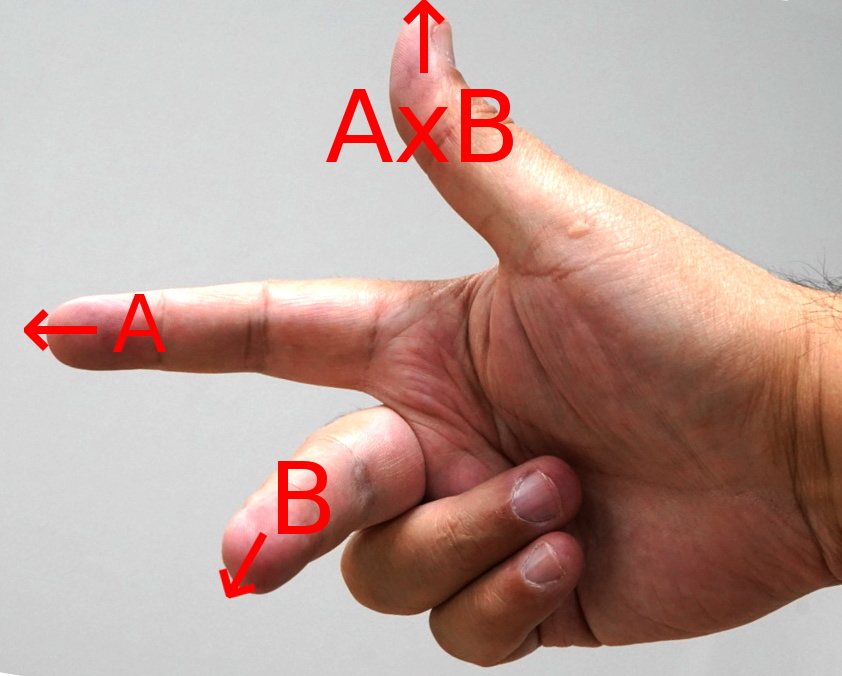
\includegraphics[height=2in]{./Chapters/Ch01-intro/righthandrule.JPG}	
	\caption{The First Right Hand Rule}
	\end{figure}
	
\end{center}

The right had rule is easiest to use when the first two vectors are at $90^\circ$ to each other.  However, even if the first two vectors are not at right angles to each other, the resultant vector of a cross product will always be perpendicular to the plane of the first two vectors.  


\newpage
\section{Exercises for Chapter 1}

\begin{multicols}{2}


	\begin{enumerate}


	\subsection*{Section 1.1: Dimensional Analysis}
		\item What are the units for each of the following?
			\begin{enumerate}
				\item $\frac{5 m}{2 s}$
				\item $\frac{10kg}{5s}$
				\item $\frac{140 kg \cdot 15 m}{23 s} $
				\item $\frac{(\frac{15m}{15s})}{14 s} $
				
			\end{enumerate}
	\subsection*{Section 1.2: Vectors and Scalars}
		\item Given the vector $4\hat{i} - 3 \hat{j}$, represent the vector (a) graphically and (b) in polar form.  
		\item George walks 200 meters north, then walks 400 meters north.  What is the vector from his starting position to his ending position in (a) cartesian form and (b) polar form (take north as 0 degrees).  
	\subsection*{Section 1.3: Vector Mathematics}
		\item Addition - cartesian
		\item Addition - polar
		\item Dot Product - Cartesian
		\item Dot Product - polar
		\item Cross Product - cartesian
		\item Cross Product - polar
		
		
	\end{enumerate}	
\end{multicols}	
	




\chapter{Kinematics in One Dimension}
\section{Distance and Displacement} \index{Distance}

You are probably already familiar with the concept of \textbf{distance} - you might get in your car and drive a total of 1.2 miles to school, turning right after 0.45 miles, according to your car's odometer.  Distance is a scalar that tells you how far something traveled.  The symbol d usually represents distance.

While you may have traveled a total distance of 1.2 miles from your school, you are significantly less than 1.2 miles away from home; in fact, you are approximately 0.874 miles from home, following a direct path directly from your home to the school, at an angle of $59^\circ $(not worrying that this path might take you through someone's back yard or kitchen).


  \textbf{Displacement} \index{Displacement} is a vector that tell you how far something is from the origin, and is independent of the path taken to get there.  The displacement vector is commonly symbolized by $\vec{r}$ though sometimes it may be written as $\vec{d}$ or $\vec{x}$. 

\section{Average and Instantaneous Speed and Velocity}

\textbf{Speed} is a scalar value that represents the change in distance per change in time of an object.  Speed is usually represented with the symbol $v$, without the vector sign.  You are probably already familiar with this quantity, since the speedometer on your family car measures speed.  For the purposes of physics, speed has little value because it is a scalar that tells us nothing of direction.  Much more useful is the concept called velocity.  Velocity and speed are related much like distance and displacement.  

\textbf{Velocity} is the change in displacement of an object per unit time, and as such is a vector.  Positive velocities indicate that the object is moving forward, relative to the axis in question, and negative velocities generally mean that the object is moving backward, relative the the axis.  The average velocity of an object is given by:
\begin{mdframed}[backgroundcolor=orange!20!white]
	\begin{equation}
	\overrightarrow{v_{avg}} = \frac{\Delta\vec{r}}{\Delta t} 
		\label{eqn:velocity}
	\end{equation}
\end{mdframed}

Average velocity is useful if an object's velocity is not changing.  However, many times it is more useful to talk about instantaneous velocity.  Instantaneous velocity tells us how fast an object is moving at a given instant in time.  In order to calculate instantaneous velocity, we must allow our time interval in the above formula to become infinitesimally small.  In this case, a little calculus proves:
\begin{mdframed}[backgroundcolor=orange!20!white]
	\begin{equation}
	\vec{v} = \frac{d\vec{r}}{dt}
	\label{equation:instantaneousvelocity}
	\end{equation}
\end{mdframed}	
	
	Calculation of average velocity is rather straightforward, assuming you know both distance traveled and the time it took.  If an object is not speeding up or slowing down during a specific time interval, the instantaneous velocity at any time during this interval is equal to the average velocity.  If the object does speed up or slow down during the time interval in question, the average velocity and the instantaneous velocity at a certain time during the interval are not necessarily the same. 
	
\begin{mdframed}[backgroundcolor=blue!10!white]
		\begin{center}


		\textbf{Example \thesection.1}	
	\end{center}

\textbf{Problem: }You ride your bicycle in a straight line for a distance of 73 meters in 12.5 second.  What is your average speed?
\vspace{0.1in}

\textbf{Solution:} 
Begin by drawing a diagram:


\begin{equation*}
 v_{avg}  = \frac{d}{t} = \frac{73m \hspace{0.05in} \hat{i}}{12.5s}  = 5.84 \frac{m}{s} \hspace{0.05in} \hat{i}
\end{equation*}

\end{mdframed}
	\vspace{0.1in}
	
\begin{mdframed}[backgroundcolor=blue!10!white]
	\begin{center}
		
		
		\textbf{Example \thesection.2}	
	\end{center}
	
	\textbf{Problem: }A bicyclist rides his bike to the east.  His position (in meters) is given by the following expression:
	\begin{equation*}
	\vec{r} = (0.5 t^2 + 4t) \hat{i}
	\end{equation*}
	\begin{enumerate}[label=\alph*.]
		\item What is his average velocity from t = 0 to t = 5 seconds?
		\item What is his instantaneous velocity at t=3 seconds?
	\end{enumerate}
	\vspace{0.1in}
	\textbf{Solution:} \begin{enumerate}[label=\alph*.]
		\item The total displacement (in meters) after five seconds is given by: 
		\begin{equation*}
		\hat{r} = (0.5 \times (5s)^2+4\times 5s) \hspace{0.05in} m \hspace{0.05in} \hat{i} = 32.5 \hspace{0.05in} m \hspace{0.05in} \hspace{0.05in} \hat{i}
		\end{equation*}
		Thus, the average velocity is - 
	\begin{equation*}
	\overrightarrow{v_{avg}}  = \frac{\vec{d}}{t} = \frac{32.5 m \hspace{0.05in} \hat{i}}{5s}  = \boxed{6.5 \frac{m}{s} \hspace{0.05in} \hat{i}}
	\end{equation*}
	
	
	
	\item The instantaneous velocity of an object is found using a derivative with respect to time.  Thus,
	
	\begin{equation*}
	\vec{v} = \frac{d\vec{r}}{dt} = \frac{d}{dt} (0.5 t^2 + 4t) \hat{i} = (t + 4) \hat{i} 
	\end{equation*}
	
	Evaluating this at t=3s yields:
	
	\begin{equation*}
	\vec{v} = (3 + 4) \hat{i} = 7 \frac{m}{s} \hat{i}
	\end{equation*}
	\end{enumerate}
	
\end{mdframed}

	
	
	
	

\section{Relative Motion at Constant Velocity}


\section{Acceleration}
\subsection{Average Acceleration} \index{Acceleration, Average}
Velocity is not always constant.  For instance, when you are driving through a city, there are times when you might be going 30 mph, and there are times when you might be stopped at a streetlight.  City driving requires you to speed up at some times, and slow down at other times – your velocity changes as a function of time.  Change in velocity per change in time is called acceleration.  
Keep in mind, both speeding up and slowing down are forms of acceleration.  In the case that an object is traveling with a positive velocity, slowing down causes negative acceleration (or deceleration).
Like velocity, acceleration comes in two basic types – average and instantaneous.  To find average velocity, we calculate the change in velocity per change in time:

\begin{mdframed}[backgroundcolor=orange!20!white]
	\begin{equation}
	\overrightarrow{a_{avg}} = \frac{\Delta \vec{v}}{\Delta t} 
	\label{equation:averageacceleration}
	\end{equation}
\end{mdframed}	
Keep in mind that this can be expressed as:
\begin{mdframed}[backgroundcolor=orange!20!white]
	\begin{equation}
	\overrightarrow{a_{avg}} = \frac{\overrightarrow{v_f} - \overrightarrow {v_i}}{\Delta t}
	\label{equation:averageaccelerationalt}
	\end{equation}
\end{mdframed}	


where $v_f$ and $v_i$ are final velocity and initial velocity, respectively.  Sometimes final velocity is expressed as $v$ and initial velocity is symbolized as $v_0$. 

\subsection{Instantaneous Acceleration} \index{Acceleration, Instantaneous}

Instantaneous velocity is found by letting the time interval in question become infinitesimally small.  A little calculus proves that:
\begin{mdframed}[backgroundcolor=orange!20!white]
	\begin{equation}
	\vec{a} = \frac{d \vec{v}}{dt} 
	\end{equation}
\end{mdframed}

Combining this with equation \ref{equation:instantaneousvelocity}, we find:
\begin{mdframed}[backgroundcolor=orange!20!white]
	\begin{equation}
	\vec{a} = \frac{d^2 \vec{r}}{dt^2} 
	\end{equation}
\end{mdframed}


\begin{mdframed}[backgroundcolor=blue!10!white]
	\begin{center}
		
		
		\textbf{Example \thesection}	
	\end{center}
	\vspace{0.1in}
	
	\textbf{Problem: } A car is traveling 20 m/s in the positive x direction.  The driver sees a red light, and applies the brakes, causing the vehicle to come to a stop in 4 seconds.  What is the average acceleration caused by the brakes?
	
	\vspace{0.1in}
	
	\textbf{Solution:} Using the definition of Average Acceleration from Equation \ref{equation:averageaccelerationalt}, we find:
	
	\begin{equation*}
			\overrightarrow{a_{avg}} = \frac{\overrightarrow{v_f} - \overrightarrow {v_i}}{\Delta t} = \frac{0 \frac{m}{s} \hat{i} - 20 \frac{m}{s} \hat{i}}{4 s}   = -5 \frac{m}{s^2} \hat{i}
	\end{equation*}
\end{mdframed}

\section{The Kinematic Equations} 
\subsection{The Kinematic Variables} \index{Kinematic Variables}
There are five variables that are often used to solve problems involving constant acceleration.  These variables are listed below:

\begin{center}
	
	
	\begin{table}[ht]\caption{\textbf{The Kinematic Variable}}% title of Table 
		\centering % used for centering table	
		\begin{tabular}{|c|c|c|}
			\hline \hline
			\textbf{Quantity} & \textbf{Variable} & \textbf{Units} \\
			\hline
			Displacement & $\vec{d}$ or $\vec{x}-\vec{x_0}$  & m \\
			\hline
			
			Initial Velocity & $\vec{v_i}$ or $\vec{v_0}$  & m/s \\
			\hline
			
			Final Velocity & $\vec{v_f}$ or $\vec{v}$  & m/s \\
			\hline
			
			Acceleration & $\vec{a}$   & $m/s^2$ \\
			\hline
			
			time & $t $  & s \\
			\hline
		\end{tabular}
		\label{table:kinematic1d}% is used to refer this table in the text
	\end{table}
\end{center}

\subsection{The Kinematic Equations}

\index{Kinematic Equations} \label{kinematicequations}
Using the definitions above, and a little calculus (or a lot of algebra) we can prove the following four equations:
\begin{mdframed}[backgroundcolor=orange!20!white]
	\begin{center}
		\textbf{The Kinematic Equations}
	\end{center}
	\begin{multicols}{2}
		\begin{equation}
		\vec{d} = \frac{\overrightarrow{v_f} + \overrightarrow{v_i}}{2}  t
		\label{equation:kinematic1}
		\end{equation}
			
		\begin{equation}
		\overrightarrow{v_f} = \overrightarrow{v_i} + \vec{a} t
		\label{equation:kinematic2}
		\end{equation}	
			
		\begin{equation}
		\vec{d} = \overrightarrow{v_i} t + \frac{1}{2}\vec{a}{t}^2
		\label{equation:kinematic3}
		\end{equation}
		
		\begin{equation}
		\overrightarrow{v_f}^2 = \overrightarrow{v_i}^2 + 2\vec{a}\vec{d}
		\label{equation:kinematic4}
		\end{equation}
		
		
			
		\end{multicols}
	\end{mdframed}

These equations enable you to solve the vast majority of kinematic problems.  Keep in mind that these equations should only be applied in one direction at at time – meaning that 2-dimensional and 3-dimensional problems will require you to split all the quantities into component vectors before you can solve these equations in each direction separately. It should also be noted that these equations assume constant acceleration.  If the acceleration of the object is changing, the equations are not valid.



\section{Vertical Motion and Gravity}

One of the most common types of acceleration we experience every day is the acceleration due to gravity.  Acceleration due to gravity is given a special symbol: g.  On Earth, $g \approx  9.81 \frac{m}{s^2}$.  Keep in mind that this value is only useful for calculations involving gravity that take place on the Earth's surface.  All planets, stars, and celestial bodies (in fact, all objects with any mass) have their own gravitational acceleration.  Acceleration due to gravity on the moon, for instance, is $1.62 \frac{m}{s^2}$.    

Objects undergo free fall when they are allowed to continue to accelerate due to gravity until they impact something that breaks their fall (often this is the ground).  In order to make the calculations easier, we often ignore air resistance.

Because gravity at the Earth's surface is downward, sign conventions become a little more important than previously.  If upward is positive, g will have a negative sign attached to it to indicate the direction of acceleration.  


\begin{mdframed}[backgroundcolor=blue!10!white]
	\begin{center}
		
		
		\textbf{Example \thesection}	
	\end{center}
	\vspace{0.1in}
	
	\textbf{Problem: } You are standing on top of a building.  You drop a rock  from the top of the building, and let it free fall until it hits the ground, 3.2 seconds later.  
	\begin{enumerate}[label=\alph*.]
		\item What is the height of the building?
		\item An identical building is build on the moon.  How long does it take the rock to fall in this case?
	\end{enumerate}

	\textbf{Solution:}
	\begin{enumerate}[label=\alph*.]
		\item To solve for distance, we apply equation 1.5.3 in the y-direction, and substitute ay = g and vi = 0 m/s,:
		
		\item Because we know that vi = 0 m/s, and ay = gm = 1.62 m/s2, we can let the final term drop out of equation 1.5.3 to yield:
	\end{enumerate}
\end{mdframed}







	

		
	







\appendix

\appendixpage
\noappendicestocpagenum
\addappheadtotoc





\chapter{Math Skills}

\section{Scientific Notation}


	\begin{itemize}
		\item Scientific Notation always has three parts: the \textit{coefficient}, the \textit{base}, and the \textit{exponent}:
		\begin{center}
			\color{blue} Coefficient $\rightarrow \color{black} 6.022 \times 10^{23 \color{red}\leftarrow}$ \textsuperscript{\color{red}Exponent} \color{black}
			
			\hspace{.7in} \color{orange}$\uparrow$
			
			\hspace{.7in} Base \color{black}
		\end{center}
		\item In scientific notation the \color{orange} base \color{black}is always 10. 
		\item A negative in front of the  \color{blue} coefficient \color{black} means the whole number is negative. 
		\item  A negative \color{red} exponent \color{black} means the number is very small (close to zero). \color{black}
		\item  The \color{red} exponent \color{black} counts how many places the decimal moved, NOT the number of zeroes.	
		\item When comparing numbers in scientific notation, look at (in order): 
		\begin{enumerate}
			\item  Negatives in front of the \color{blue} coefficient. \color{black}
			\item \color{red}Exponents \color{black}
			\item \color{blue}Coefficients \color{black}
		\end{enumerate}
		
		\item To multiply, multiply coeffients, then ADD exponents.
		\item To divide, divide coefficients, then SUBTRACT exponents.
		\item To raise to a power, raise the coefficient to the power, then MULTIPLY exponents.
		\item To enter scientific notation on most calculators use the ``EE" key. $6.022 \times 10^{23}$ is entered as 6.022\scriptsize E\normalsize23.  Calculator notation should \underline{\textbf{never}} be handwritten. 
		\item Metric Prefixes are really just scientific notation:
		\begin{center}
			\begin{tabular}{|c|c|c|}
				\hline
				Prefix & Letter & Power of 10 \\
				\hline
				nano & n &  $ \times 10^{-9}$ \\
				\hline
				micro & $\mu$ &  $ \times 10^{-6}$ \\
				\hline
				milli & m & $ \times 10^{-3}$ \\
				\hline
				centi & c & $ \times 10^{-2}$ \\
				\hline
				deci & d & $ \times 10^{-1}$ \\
				\hline
				Deka & D & $ \times 10^{1}$ \\
				\hline
				Hecto & H & $ \times 10^{2}$ \\
				\hline
				Kilo & k & $ \times 10^{3}$ \\
				\hline
				Mega & M & $ \times 10^{6}$ \\
				\hline
				Giga & G & $ \times 10^{9}$ \\
				\hline
				
			\end{tabular}	
		\end{center}
		
		
	\end{itemize}
\newpage

\section{Algebra}
To study physics, you should have some knowledge of algebra. Though this appendix is too small to include all algebraic techniques, there are some things that are repeated often in physics. These commonly recurring algebraic themes are highlighted here.

\subsection{Solve for a Variable}

Solving for a variable is one of the most fundamental skills in algebra and physics. Whether you're isolating a variable to find a force, velocity, or time, this process involves rearranging equations using inverse operations.



\begin{mdframed}[backgroundcolor=blue!10!white]
	\begin{center}
		
		
		\textbf{Example \thesection.1}	
	\end{center}
	
	\textbf{Problem:} Solve the Equation \color{blue}$2x+3 = 12x +1$  \color{black} for \color{blue}$x$\color{black}.
	\vspace{0.1in}
	
	\textbf{Solution:} To solve this equation, we begin by combining like terms.  Terms involving \color{blue}$x $ \color{black} should be moved to one side, while terms involving only numbers are moved to the other.  
	\color{blue}
	
	\begin{equation*}
		2x + 3 = 12 x +1
	\end{equation*}
	\begin{equation*}
	-10x +3  = 1
\end{equation*}
	\begin{equation*}
	-10x = -2
\end{equation*}
\color{black}


Now, dividing by -10 gives: 
	\color{blue}
	\begin{equation*}
	x = 5
\end{equation*}	
	\color{black}
\end{mdframed}
\newpage

\subsubsection{Solve for a Variable in the Denominator of a Fraction}

Sometimes, the variable you're solving for appears in the denominator. This can often be confusing at first, but the trick is to eliminate the fraction by multiplying both sides by the denominator.

\begin{mdframed}[backgroundcolor=blue!10!white]
	\begin{center}
	
	
	\textbf{Example \thesection.1.2}	
\end{center}

\textbf{Problem:} Solve for \( R \) in the equation:

	\begin{equation*}
			V = \frac{I}{R}
	\end{equation*}

	


\textbf{Solution:} Multiply both sides by \( R \) to eliminate the denominator:
\[
V \cdot R = I
\]
Then divide both sides by \( V \) to isolate \( R \):
\[
R = \frac{I}{V}
\]

\end{mdframed}

\subsubsection{Solve for a Variable using the Quadratic Formula} \index{Quadratic Forumula}

In some physics problems, especially those involving kinematics or energy, you might encounter equations that take the form of a quadratic:

\[
ax^2 + bx + c = 0
\]

The solution is given by the quadratic formula:
\[
x = \frac{-b \pm \sqrt{b^2 - 4ac}}{2a}
\]

\begin{mdframed}[backgroundcolor=blue!10!white]
	\begin{center}
		
		
		\textbf{Example \thesection.1.3}	
	\end{center}
	
	\textbf{Problem:}
	Solve for \( t \):
	\[
	0 = 5t^2 - 20t + 15
	\]


\textbf{Solution:} Identify \( a = 5 \), \( b = -20 \), and \( c = 15 \). Plug into the quadratic formula:

\[
t = \frac{-(-20) \pm \sqrt{(-20)^2 - 4(5)(15)}}{2(5)} = \frac{20 \pm \sqrt{400 - 300}}{10} = \frac{20 \pm \sqrt{100}}{10}
\]

\[
t = \frac{20 \pm 10}{10} = 3 \text{ or } 1
\]

It should be noted that negative answers can arise in physics, and negatives often indicate direction.  However, context tells you which solutions are meaningful.  While a negative velocity may just mean an object is traveling opposite the expected direction, a negative time is likely meaningless.

\end{mdframed}
\newpage

\subsection{Solve a System of Equations}

Many physics problems involve more than one equation and variable. These systems can be solved using several algebraic techniques.

\subsubsection{Solve a System of Equations by Combination}

Also called the addition or elimination method, this approach involves adding or subtracting equations to eliminate one variable.  This is particularly useful when coefficients are opposites or can easily be made opposites.

\begin{mdframed}[backgroundcolor=blue!10!white]
	\begin{center}
		
		
		\textbf{Example \thesection.1.4}	
	\end{center}
	
	\textbf{Problem:}
	Solve the system:
	\[
	\begin{aligned}
		2x + 3y &= 12 \\
		4x - 3y &= 6
	\end{aligned}
	\]


\textbf{Solution:} Add the equations to eliminate \( y \):
	\[
\begin{aligned}
	2x + 3y &= 12 \\
	+  \hspace{0.1in} 4x - 3y &= 6\\
	\hline
	6x \hspace{0.3in} &= 18 \\
	x&=3
\end{aligned}
\]

Substitute \( x = 3 \) into the first equation:
\[
2(3) + 3y = 12 \Rightarrow 6 + 3y = 12 \Rightarrow y = 2
\]


\end{mdframed}

\newpage
\subsubsection{Solve a System of Equations by Substitution}

This method is ideal when one of the equations is already solved for one variable, or can easily be rearranged to do so. 

\begin{mdframed}[backgroundcolor=blue!10!white]
	\begin{center}
		
		
		\textbf{Example \thesection.1.5}	
	\end{center}
	
	\textbf{Problem:}
	Solve the system:
	\[
	\begin{aligned}
		y &= 2x + 1 \\
		3x + y &= 16
	\end{aligned}
	\]


\textbf{Solution:} Substitute the expression for \( y \) into the second equation:
\begin{equation*}
3x + (2x + 1) = 16 	
\end{equation*}
\begin{equation*}
	 5x + 1 = 16 
\end{equation*}
\begin{equation*}
	 5x = 15
	 \end{equation*}
 \begin{equation*}
 	x = 3
 \end{equation*} 

Now substitute back to find \( y \):
\[
y = 2(3) + 1 = 7
\]

\end{mdframed}

\newpage
\subsubsection{Solve a System of Equations using Matrices}

Matrices are useful for solving larger systems of equations, especially in physics problems involving circuits or forces in multiple directions.  If you have three or more variables an equal number of equations, using a matrix to solve the problem keeps your work organized as well.  You may use any of the following operations:
\begin{itemize}
	\item Multiply or divide any row by a constant.
	\item Add two rows together, and replace either row with the result.
	\item Swap the order of rows.
\end{itemize}


\begin{mdframed}[backgroundcolor=blue!10!white]
	\begin{center}
		
		
		\textbf{Example \thesection.1.5}	
	\end{center}
	
	\textbf{Problem:}

	Solve the system using matrices:
\begin{equation*}
	\begin{aligned}
	2x + 3y + z &= 8 \\
	x + y - z &= 1 \\
	3x + 2y + z &= 15
\end{aligned}
\end{equation*}


\textbf{Solution:} Begin by writing the equations as an augmented matrix: 
\vspace{-0.2in}

	\begin{equation*}
\begin{bmatrix}
	2 & 3 & 1 & 8 \\
	1 & 1 & -1 & 1\\
	3 & 2 & 1 & 15 
\end{bmatrix} 		
	\end{equation*}

First, we can multiply the 2nd row by -2.

	\begin{equation*}
		R_2 = -2 R_2 \longrightarrow
	\begin{bmatrix}
		2 & 3 & 1 & 8 \\
		-2 & -2 & 2 & -2\\
		3 & 2 & 1 & 15 
	\end{bmatrix} 		
\end{equation*}

Now we add Row 1 to Row 2:

\begin{equation*}
	R_2 = R_1 + R_2 \longrightarrow
	\begin{bmatrix}
		2 & 3 & 1 & 8 \\
		0 & 1 & 3 & 6\\
		3 & 2 & 1 & 15 
	\end{bmatrix} 		
\end{equation*}

Next, we multiply Row 1 by 3 and row 3 by -2:

\begin{equation*}
	\begin{aligned}
		R_1 &= 3 R_1 \\
		R_3 &= -2 R_3
	\end{aligned}
	\longrightarrow
	\begin{bmatrix}
		6 & 9 & 3 & 24 \\
		0 & 1 & 3 & 6\\
		-6 & -4 & -2 & -30 
	\end{bmatrix} 		
\end{equation*}

Now we can add Row 1 to Row 3:
\begin{equation*}
	R_3 = R_1 + R_3
	\longrightarrow
\begin{bmatrix}
	6 & 9 & 3 & 24 \\
	0 & 1 & 3 & 6\\
	0 & 5 & 1 & -6 
\end{bmatrix} 	
\end{equation*}

Multiplying row 2 by -5 gives:
\begin{equation*}
	R_2 = -5R_2
	\longrightarrow
	\begin{bmatrix}
		6 & 9 & 3 & 24 \\
		0 & -5 & -15 & -30\\
		0 & 5 & 1 & -6 
	\end{bmatrix} 	
\end{equation*}

Adding Row 2 and row 3 yields:
\begin{equation*}
	R_3 = R_2 + R_3
	\longrightarrow
	\begin{bmatrix}
		6 & 9 & 3 & 24 \\
		0 & -5 & -15 & -30\\
		0 & 0 & -14 & -36 
	\end{bmatrix} 	
\end{equation*}

Now we can divide Row 3 by -14:

\begin{equation*}
	R_3 = \frac{R_3}{-14}
	\longrightarrow
	\begin{bmatrix}
		6 & 9 & 3 & 24 \\
		0 & -5 & -15 & -30\\
		0 & 0 & 1 & \frac{18}{7} 
	\end{bmatrix} 	
\end{equation*}

This means that $z = \frac{18}{7}$.  Continuing to solve the problem, we can multiply row 3 by 15 and add it to row 2 to to get: 

\begin{equation*}
	R_2 = R_2 + 15 R_3  
	\longrightarrow
	\begin{bmatrix}
		6 & 9 & 3 & 24 \\
		0 & -5 & 0 & \frac{60}{7}\\
		0 & 0 & 1 & \frac{18}{7} 
	\end{bmatrix} 	
\end{equation*}

Now, divide row 2 by -5:

\begin{equation*}
	R_2 = \frac{R_2}{5}   
	\longrightarrow
	\begin{bmatrix}
		6 & 9 & 3 & 24 \\
		0 & 1 & 0 & \frac{-12}{7}\\
		0 & 0 & 1 & \frac{18}{7} 
	\end{bmatrix} 	
\end{equation*}

Which means we now know $y = \frac{-12}{7}$.  We can now use row 2 and row 3 to eliminate variables in row 1:  

\begin{equation*}
	R_1 = R1 + (-9 R_2) + (-3 R_3)  
	\longrightarrow
	\begin{bmatrix}
		6 & 0 & 0 & \frac{222}{7} \\
		0 & 1 & 0 & \frac{-12}{7}\\
		0 & 0 & 1 & \frac{18}{7} 
	\end{bmatrix} 	
\end{equation*}

Finally, dividing Row 1 by 6 gives: 
\begin{equation*}
	R_1 = \frac{R_1}{6}
	\longrightarrow
	\begin{bmatrix}
		1 & 0 & 0 & \frac{37}{7} \\
		0 & 1 & 0 & \frac{-12}{7}\\
		0 & 0 & 1 & \frac{18}{7} 
	\end{bmatrix} 	
\end{equation*}


\end{mdframed}



\newpage
\section{Proportional Reasoning}
\subsection{Proportional Reasoning}

Proportional reasoning is a powerful tool in physics. Often, you don’t need to plug in numbers to figure out how a change in one variable affects another. You only need to understand how variables are related in a formula.

\textbf{The idea:} If a formula contains multiple variables, and you know how one variable changes, you can predict how the output will change—assuming all other variables stay constant or have known changes.


	The force of gravity between two masses is given by:
	\[
	F = G \frac{m_1 m_2}{r^2}
	\]
	A planet has twice Earth’s mass and three times Earth’s radius. If the gravitational force on a mass on Earth is \( F_E \), what is the gravitational force on the same mass on the new planet, in terms of \( F_E \)?


\textbf{Solution:} Let Earth have mass \( M \), and radius \( R \), so:
\[
F_E = G \frac{m M}{R^2}
\]

On the new planet:
\[
F' = G \frac{m (2M)}{(3R)^2} = G \frac{2mM}{9R^2} = \frac{2}{9} F_E
\]

\textbf{Answer:} \( \frac{2}{9} F_E \)

\textbf{Comment:} The trick is to substitute the new values into the formula and simplify. Don’t calculate anything you don’t need.

\vspace{1em}

	The period \( T \) of a pendulum is given by:
	\[
	T = 2\pi \sqrt{\frac{L}{g}}
	\]
	If the length \( L \) of a pendulum is quadrupled, by what factor does the period \( T \) change?


\textbf{Solution:}
\[
T' = 2\pi \sqrt{\frac{4L}{g}} = 2\pi \cdot 2\sqrt{\frac{L}{g}} = 2T
\]

\textbf{Answer:} The period doubles.

\textbf{Comment:} When a variable is inside a square root, its effect is weaker. Quadrupling \( L \) only doubles \( T \).

\vspace{1em}

	The kinetic energy of an object is:
	\[
	K = \frac{1}{2}mv^2
	\]
	If the velocity of the object triples, how does its kinetic energy change?


\textbf{Solution:}
\[
K' = \frac{1}{2} m (3v)^2 = \frac{1}{2} m \cdot 9v^2 = 9K
\]

\textbf{Answer:} The kinetic energy increases by a factor of 9.

\textbf{Comment:} Pay attention to exponents—tripling \( v \) squares the effect in \( v^2 \).

\vspace{1em}

	The electric force between two charges is given by:
	\[
	F = k \frac{q_1 q_2}{r^2}
	\]
	If both charges are doubled and the distance is halved, what happens to the electric force?


\textbf{Solution:}
\[
F' = k \frac{(2q_1)(2q_2)}{(r/2)^2} = k \frac{4q_1 q_2}{r^2/4} = k \frac{4q_1 q_2 \cdot 4}{r^2} = 16F
\]

\textbf{Answer:} The force increases by a factor of 16.

\textbf{Comment:} Changing more than one variable? Just multiply each effect together.

\vspace{1em}

	The pressure at the bottom of a fluid is given by:
	\[
	P = \rho g h
	\]
	If the height of the fluid is doubled and the fluid is twice as dense, what happens to the pressure?


\textbf{Solution:}
\[
P' = (2\rho) g (2h) = 4 \rho g h = 4P
\]

\textbf{Answer:} The pressure increases by a factor of 4.

\textbf{Comment:} Linear relationships like this are easy to reason through—just multiply the scaling factors.


\newpage
\section{Trigonometry}

\newpage
\section {Radians and Arc Length}
\subsection{Radians} \index{Radians}

Just like there are many different units that measure distance (meters, feet, inches, miles, furlongs, etc.), there are also different ways of measuring angles.  You are probably already familiar with degrees. A right angle is $90 \degree$, and a full circle is $360 \degree$.  When calculating arc length or using the angular kinematic equations, the standard units for angles are \textit{radians}\footnote{It should be noted that strictly speaking, radians are not a unit; since the definition of a radian has to do with a ratio, all numbers with radians as the unit are actually unitless.}  There are $2 \pi$ radians in a complete circle, so,

	\begin{mdframed}[backgroundcolor=green!20!white]
	\begin{equation*}
		360 \degree = 2 \pi \, \si{radians}
		\label{conversion:radiandegree}
	\end{equation*}
\end{mdframed}	

This equation can be used to convert an angle from radians to degrees or vice-versa.  

 \begin{mdframed}[backgroundcolor=blue!10!white]
	\begin{center}	
		\textbf{Example \thesection.1}	
	\end{center}
	
	\textbf{Problem:} An angle measures $34 \degree$.  What is this angle in radians? 
	
	\vspace{0.2 in} 
	\textbf{Solution}: Begin by creating a conversion factor.  In this case, since we have degrees and want radians, we create a fraction with $2\pi$ radians on top of the fraction, and $360\degree$ on the bottom.  Multiplying by this fraction gives:
	
\begin{equation*}
	34 \degree \times \frac{2 \pi \, \si{rad}}{360 \degree} = \frac{17 \pi}{90}\si{rad} \approx 0.593 \, \si{rad}  
\end{equation*}
	
	It should be noted that the fraction $\frac{2 \pi \, \si{rad}}{360 \degree}$ can easily be reduced to $\frac{ \pi \, \si{rad}}{180 \degree}$ .  Using this as your conversion factor will yield the same results.  It is also often easier and more accurate to leave measurements involving radians in terms of $\pi$.  
	
\end{mdframed}
   
   
    \begin{mdframed}[backgroundcolor=blue!10!white]
   	\begin{center}	
   		\textbf{Example \thesection.2}	
   	\end{center}
   	
   	\textbf{Problem:} An angle measures $\frac{\pi}{2} \si{rad}$.  What is this angle in degrees? 
   	
   	\vspace{0.2 in} 
   	\textbf{Solution}: Again, we begin by creating a conversion factor.  Because we have a measurement in radians and are asked to find degrees, we create a fraction with $360\degree$ on top of the fraction, and  $2\pi$ radians on the bottom:
   	
   	\begin{equation*}
   		\frac{\pi}{2}  \times \frac{360 \degree}{2 \pi \, \si{rad}} = 90 \degree
   	\end{equation*}
 
   	
   \end{mdframed}

\newpage
   \subsection{Arc Length} \index{Arc Length}
   
   The distance along the circumference of a circle that corresponds to an internal angle of the circle is called \textit{Arc Length}.  Though arc-length is a measurement of length, the symbol used for Arc Length is $s$. 
 \begin{figure}[h]
 	  \begin{center}
   	 	\begin{tikzpicture}
   		% the origin
   		\coordinate (O) at (0,0);
   		% the circle and the dot at the origin
   		\draw (O) node[circle,inner sep=1.5pt,fill] {} circle [radius=3cm];
   		% the ``\theta'' arc
   		\draw 
   		(3 cm,0) coordinate (xcoord) -- 
   		node[midway,below] {$r$} (O) -- 
   		(60:3 cm) coordinate (slcoord)
   		pic [draw,->,angle radius=1cm,"$\theta$"] {angle = xcoord--O--slcoord};
   		% the outer ``s'' arc
   		\draw[|-|]
   		(3 cm +10pt,0)
   		arc[start angle=0,end angle=60,radius=3cm+10pt]
   		node[midway,fill=white] {$s$};
   	\end{tikzpicture}
   \end{center}
 \caption{The relationship between arc-length, radius, and angle}
 \end{figure}
   	
  
   	

   
   
   
   
   
   
   
   
   
    Arc Length can be found using the following equation:
   
   	\begin{mdframed}[backgroundcolor=orange!20!white]
   	
   	\begin{equation}
   		s = r \theta
   		\label{equation:arclength}
   	\end{equation}
   \end{mdframed}
where $r$ is the radius of the circle and $\theta$ is the internal angle, measured in radians. Additionally, while meters are the proper SI units for these measurements, this formula will work with any units of length as long as both arc-length, $s$, and radius, $r$ are measured using the same units.  




\newpage

  \begin{mdframed}[backgroundcolor=blue!10!white]
	\begin{center}	
		\textbf{Example \thesection.2}	
	\end{center}
	
	\textbf{Problem:} Find the arc length of $30\degree$ of a circle with a radius of 0.2 meters.  
	 
	
	\vspace{0.2 in} 
	\textbf{Solution}: Begin by drawing a diagram:
	
	
	 	  \begin{center}
		\begin{tikzpicture}
			% the origin
			\coordinate (O) at (0,0);
			% the circle and the dot at the origin
			\draw (O) node[circle,inner sep=1.5pt,fill] {} circle [radius=3cm];
			% the ``\theta'' arc
			\draw 
			(3 cm,0) coordinate (xcoord) -- 
			node[midway,below] {$0.2 \si{m}$} (O) -- 
			(30:3 cm) coordinate (slcoord)
			pic [draw,->,angle radius=1.6cm,"$30 \degree$"] {angle = xcoord--O--slcoord};
			% the outer ``s'' arc
			\draw[|-|]
			(3 cm +10pt,0)
			arc[start angle=0,end angle=30,radius=3cm+10pt]
			node[midway,fill=blue!10!white] {$s$};
		\end{tikzpicture}
	\end{center}

	In order to find arc length, we must first convert the angle from degrees to radians:
	\begin{equation*}
	\theta = 30 \degree \times \frac{2 \pi \si{rad}} {360 \degree} = \frac{\pi}{6} \si{rad}
	\end{equation*}
	
	Now, arc length can be found using equation \ref{equation:arclength}.
	\begin{equation*}
		s = r \theta = (0.2 \si{m})(\frac{\pi}{6} \si{rad}) \approx 0.105 \si{m}
	\end{equation*}
	
	
\end{mdframed}
  



\chapter{Reference Tables}
\section{Greek Letters}
\index{Greek Letters}
\begin{longtable}{| c  | c | c | c |}
	\hline
	\textbf{Name} & \textbf{Captial} & \textbf{Lower Case} & \textbf{Alternate versions} \\
	\hline
	alpha	& $ A $ & $\alpha$ & \\
	\hline
	beta & B & $\beta$  & \\
	\hline
	gamma & $\Gamma $ & $\gamma$ & \\
	\hline
	delta & $\Delta$ & $ \delta $ & \\
	\hline
	epsilon & E & $\varepsilon $ & $\epsilon $\\
	\hline
	zeta & Z & $\zeta $ & \\
	\hline
	eta & H & $\eta$ & \\
	\hline
	theta & $\Theta$ & $\theta$ & $\varTheta$, $\vartheta$\\
	\hline
	iota & I & $\iota$ &  \\
	\hline
	kappa & K& $\kappa$ & \\
	\hline
	lambda & $\Lambda $ & $\lambda$ & $\varLambda$ \\
	\hline
	mu & M & $\mu$ & \\
	\hline
	nu & N & $\nu$ & \\
	\hline
	xi & $\Xi$ & $\xi$ & $\varXi $ \\
	\hline
	omicron & O & o & \\
	\hline
	pi & $\Pi$ & $\pi$ & $\varPi \varpi$ \\
	\hline
	rho & P & $\rho$ & $\varrho$ \\
	\hline
	sigma & $\Sigma$ & $\sigma$, $\varsigma$ & \\ 
	\hline
	tau & T & $\tau$ & \\
	\hline
	upsilon & $\Upsilon$ & $\upsilon$ & $\varUpsilon$\\
	\hline
	phi & $\Phi$ & $\phi$ & $\varPhi$, $\varphi$ \\
	\hline
	chi & X & $\chi$ &  \\
	\hline
	psi & $\Psi$ & $\psi$ &  $ \varPsi$\\
	\hline
	omega & $\Omega$ & $\omega$ & $\varOmega $ \\
	\hline
\end{longtable}

\newpage

\section{Musical Notes and Frequencies}

\index{Frequencies of Musical Notes}


\begin{center}

	
	\begin{table}[h]
		\caption{\label{tab:Frequencies}Frequencies of Musical Notes, in Hz}	
		\begin{tabular}{ |c | c | c | c | c | c | c | c | c |c|}
		
			\hline 
			\textbf{Octave:} & 0 & 1 & 2 &3&4&5&6&7&8 \\
			\hline 
			C & 16.35 & 32.70 & 65.41 & 130.81 & 261.63 & 523.25 & 1046.50 & 2093.00 & 4186.01 \\
			\hline
			C$\sharp$/D$\flat$& 17.32 & 34.65 & 69.30 & 138.59& 277.18 & 554.37 & 1108.733 & 2217.46 & 4434.92 \\
			\hline
			D & 18.35 & 36.71 & 73.42 & 146.83 & 293.66 & 587.33 & 1174.66 & 2349.32 & 4698.64 \\
			\hline
			D$\sharp$/E$\flat$& 19.45 &38.89 & 77.78& 155.56& 311.13& 622.25 & 1244.51& 2489.02& 4978.03 \\
			\hline
			E &	20.60&41.20&82.41&164.81&329.63&659.26&1318.51&2637.02&5274.04\\
			\hline
			F  & 21.83&	43.65&	87.31&	174.61&	349.23&	698.46&	1396.91&	2793.83& 5587.65 \\
			\hline
			F$\sharp$/G$\flat$& 23.12&	46.25&92.50& 185.00&369.99&	739.99&	1479.98&2959.96&5919.91 \\
			\hline
			G & 24.50&49.00&98.00&196.00&392.00&783.99&1567.98&3135.96&6271.93\\
			\hline
			G$\sharp$/A$\flat$& 25.96&51.91&103.83&207.65&415.30&830.61&1661.22&3322.44&6644.88\\
			\hline
			A &27.50&55.00&110.00&220.00&440.00&880.00&1760.00&3520.00&7040.00\\
			\hline
			A$\sharp$/B$\flat$ & 29.14&58.27&116.54&233.08&466.16&	932.33&1864.66&3729.31&7458.62\\
			\hline
			B& 30.87&61.74&123.47&246.94&493.88&987.77&1975.53&3951.07&7902.13\\
			\hline			
		\end{tabular}
	\end{table}
\end{center}

\section{Densities of Common materials}
\index{Densities, of common materials}


	The table below shows the density of some common materials:
\begin{center}
	\begin{table}[h]
			\caption{\label{tab:density}Table of Densities of Common Materials}
	\begin{longtable}{|c|c|} 
		\hline
		\textbf{Material} & \textbf{Density} ($\frac{kg}{m^3}$) \\
		\hline
		Ethanol &  789 \\
		\hline
		Ice &  917 \\
		\hline
		Olive Oil & 929 \\
		\hline
		Water (pure) & 1000 \\
		\hline 
		Water (ocean) & 1025 \\
		\hline
		
		
		
	\end{longtable}
\end{table}
\end{center}

\section{Common Indices of Refraction}
\index{Index of Refraction, Table of Common}
\begin{center}



	\begin{table}[h]
	\caption{\label{tab:refraction}Table of Common Indices of Refraction}
	
	\begin{longtable}{|c |c|}
		\hline
		\textbf{Material} & \textbf{Index of Refraction} \\
		\hline
		Air & 1.000273 \\
		\hline
		Acrylic & 1.495 \\
		\hline
		Cubic Zirconium & 2.15-2.18\\
		\hline
		Diamond & 2.417 \\
		\hline
		Crown Glass & 1.485-1.755\\
		\hline
		Flint Glass & 1.60-1.62 \\
		\hline
		Vacuum (Empty Space) & 1 \\
		\hline
		Vegetable Oil &1.47 \\
		\hline
		Water & 1.333 \\		
		\hline

	\end{longtable}


\end{table}
\end{center}
Source: Wikipedia contributors. (2021, January 8). \href{https://en.wikipedia.org/wiki/List_of_refractive_indices}{List of refractive indices}. In Wikipedia, The Free Encyclopedia


\newpage




\begin{table}[h]
	\caption{\label{tab:specificheat}Table of Specific Heat Capacities of Common Materials}
	
	\begin{longtable}{|c |c|}
		\hline
		Material & Specific Heat Capacity  \\
		\hline
		ice & df \\
		\hline
		water & 34  \\
		\hline
		Water Vapor &  43 \\
		\hline
		
	\end{longtable}
\end{table}
 \newpage




\section{Physical Constants}
\index{Physical Constants}

\
\begin{table}[h]
	\caption{\label{tab:Constants}Table of Common Physical Constants}
	
	\begin{longtable}{|c |c| c |}
		\hline
		Quantity & Symbol & Value \\
		\hline
		Boltzman's Constant & $k_B$ & 	$1.380649 \times 10^{-23}\si{\frac{J}{K}}$ \\
		\hline
		Coulomb's Constant & $k$ & $8.98755179 \times 10^9\si{\frac{kg m^2}{C^2}}$ \\
		\hline
		Charge of an electron & $e^-$ & $1.6 \times 10^{-19}\si{C}$ \\
		\hline
		Gas Constant & $R$ &  $ \SI{8.31446261815324}{\frac{J}{mol\cdot K}} $\\
		\hline
		Speed of light & $c$ & $2.99792458 \times 10^8 \si{m/s}$ \\
		\hline
		Universal Gravitational Constant &  $G$ & $6.67 \times 10^{-11} \si{\frac{Nm^2}{kg^2}}$ \\
		\hline
	
	\end{longtable}
\end{table}


		
	\backmatter	
	
\printindex		








\end{document}